\documentclass[11pt,letterpaper]{report}
\usepackage[latin1]{inputenc}
\usepackage{amsmath}
\usepackage{amsfonts}
\usepackage{amssymb}
\usepackage{graphicx}
\usepackage{color}
\usepackage{enumitem}
\usepackage[dvipsnames]{xcolor}
\definecolor{codegray}{gray}{0.9}
\newcommand{\code}[1]{\colorbox{codegray}{\texttt{#1}}}
\graphicspath{{./images/}{IR}}
%\newcommand{\LF}{}  % turn on to display large format
\ifdefined \LF
\usepackage[left=2.0cm, top=2.0cm, landscape]{geometry}  % for large format landscape
\else
\usepackage[left=2.0cm, top=2.0cm]{geometry}
\fi
\usepackage{fancyhdr}
\pagestyle{fancy}
\fancyhead{}
\lhead{CS333}
\chead{Project 2 Test Report}
\rhead{Alexander DuPree}
\begin{document}
\title{Project 2 Test Report}
\author{Alexander DuPree}

\ifdefined \LF
{\Large     % large print start
\fi

  \maketitle
  \section*{Introduction}
  \noindent
  The following test report documents the tests performed for project two. The test cases and strategies closely follow the project two rubric. 

  Each section contains test cases related to the sections topic. Each test case will describe the name of the test, 
  the expected result, actual result, as well as a discussion and indication of the Pass/Fail status. 
  The actual result will be provided in the form of a screen shot of the console. 

  \section*{Compilation}
  This section presents all tests related to compiling the xv6 kernel.
  Test cases follow closely those outlined in the rubric. \hfill \break
  
  \noindent\textbf{Test Case:} \emph{With CS333\_PROJECT set to 0 in the Makefile}
  
  \noindent\textbf{Assertions:}
  \begin{enumerate}[]
  \item Code correctly compiles
  \item Kernel successfully boots
  \end{enumerate}  
  
  \noindent\textbf{Status:} \textcolor{ForestGreen}{\textbf{PASS}}
  
  \begin{figure}[h!]
	\centering
	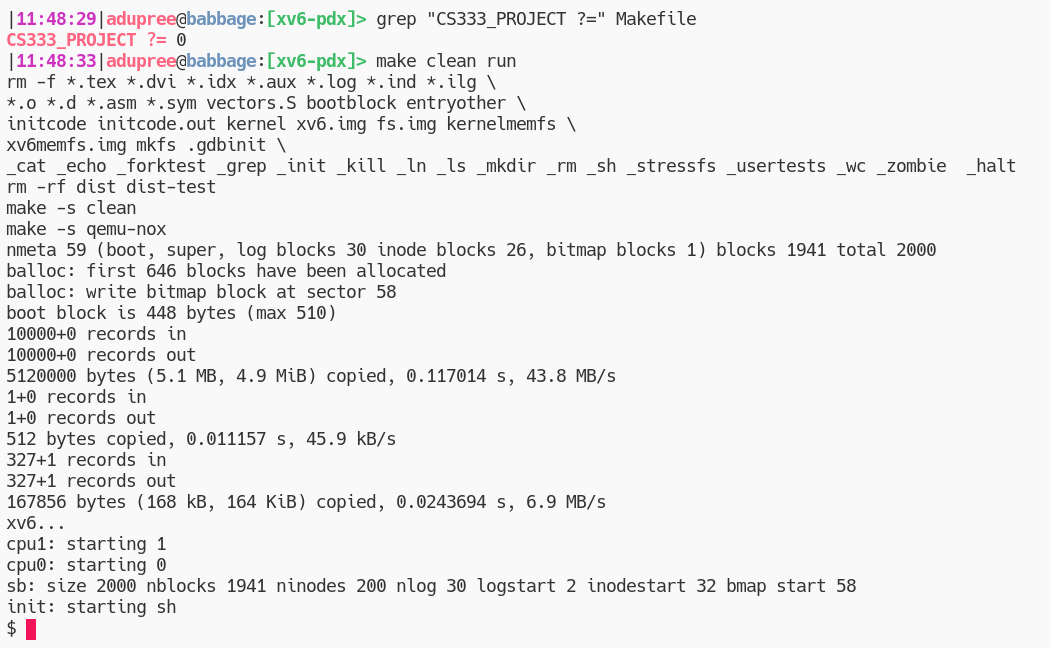
\includegraphics[width=1\linewidth]{compilation1.png}
	\caption[img]{Compilation and boot with CS333\_PROJECT set to 0.}
	\label{fig:P1compileP0-1}
  \end{figure}

  The command \code{grep "CS333\_PROJECT ?=" Makefile} shows that the CS333\_PROJECT macro is set to 0.
  The following command \code{make clean run} demonstrates that the code correctly compiles and the kernel successfully boots. 
  Furthermore, the commands were executed within seconds of each other, indicating that
  tampering is not a possibility.\\

  \noindent\textbf{Test Case:} \emph{With CS333\_PROJECT set to 2 in the Makefile}
  
  \noindent\textbf{Assertions:}
  \begin{enumerate}[]
  \item Code correctly compiles
  \item Kernel successfully boots
  \end{enumerate}  
  
  \noindent\textbf{Status:} \textcolor{ForestGreen}{\textbf{PASS}}
  
  \begin{figure}[h!]
	\centering
	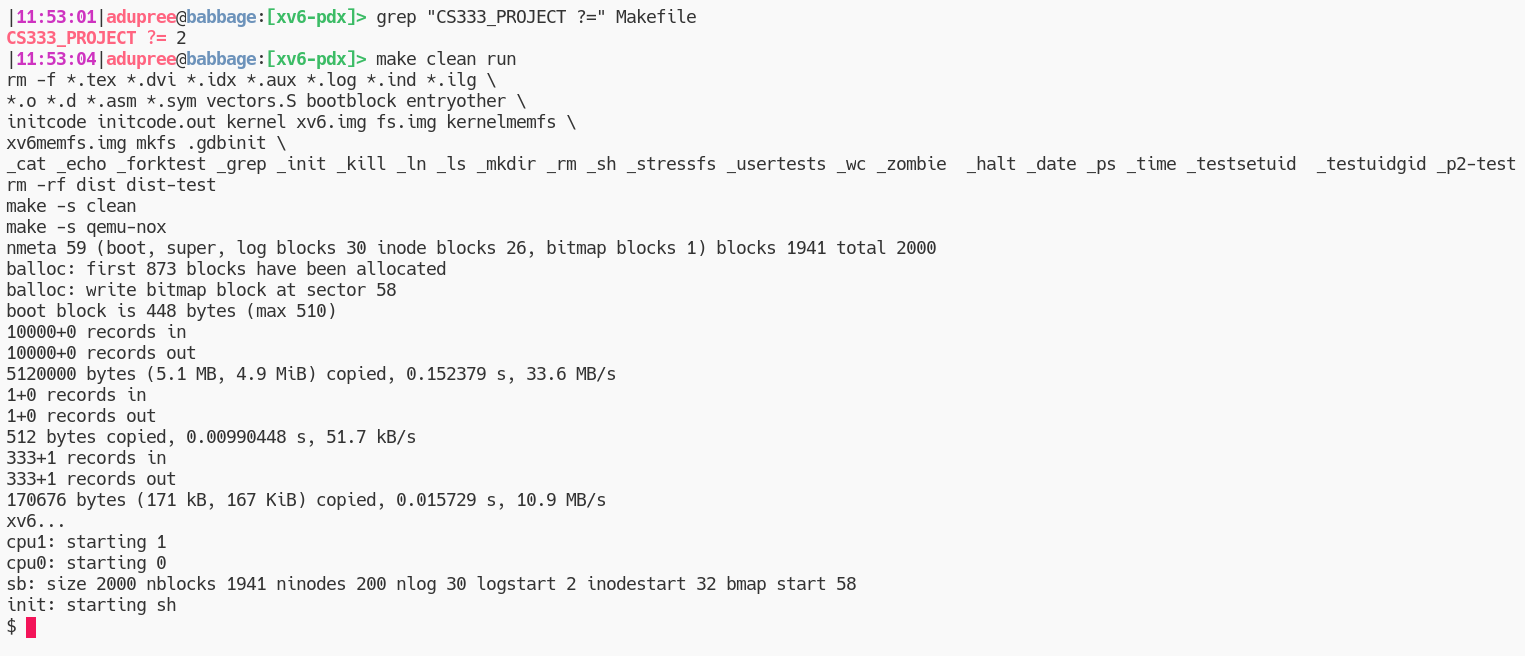
\includegraphics[width=1\linewidth]{compilation2.png}
	\caption[img]{Compilation and boot with CS333\_PROJECT set to 2, CS333\_P2 is defined.}
	\label{fig:P1compileP0-1}
  \end{figure}

  The command \code{grep "CS333\_PROJECT ?=" Makefile} shows that the CS333\_PROJECT macro
  is indeed set to 2. The following command \code{make clean run} demonstrates that the code
  correctly compiles and the kernel successfully boots. Furthermore, the commands were executed
  within seconds of each other, indicating that tampering is not a possibility. 

  \pagebreak

  \section*{PS program, CTRL-P, CPU time, getprocs() system call}
  This section presents all tests related to the \code{ps} user program, \code{CTRL+P}
  interrupt, and the \code{getprocs()} system call. 
  Test cases follow closely those outlined in the rubric. \hfill \break
  
  \noindent\textbf{Test Case:} \emph{Running the PS program}
  
  \noindent\textbf{Assertions:}
  \begin{enumerate}[]
  \item Correctly displays process information
  \item Elapsed CPU time is correct and formatted correctly
  \item Information closely matches the \code{CTRL+P} interrupt
  \item PS does not display \code{EMBRYO} or \code{UNUSED} processes
  \item \code{getprocs()} copies process info into the user space up to the number of processes or to the size of the given table
  \end{enumerate}  
  
  \noindent\textbf{Status:} \textcolor{ForestGreen}{\textbf{PASS}}
  
  \begin{figure}[h!]
	\centering
	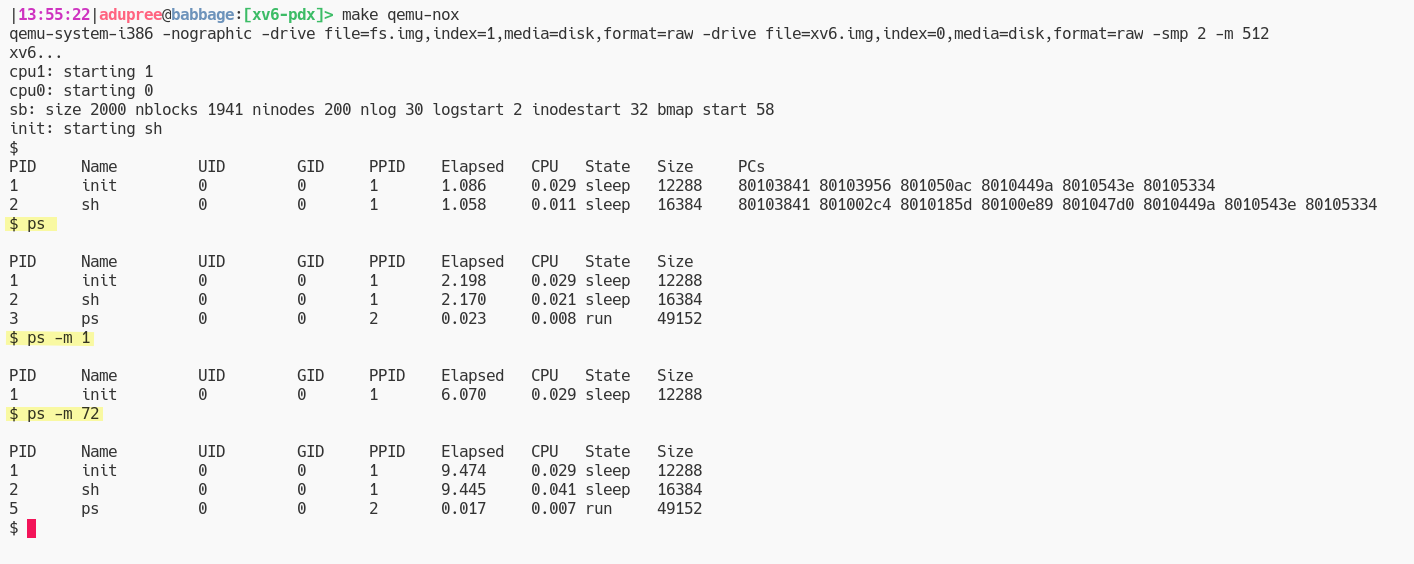
\includegraphics[width=1\linewidth]{ps-test.png}
	\caption[img]{Compilation and boot with CS333\_PROJECT set to 0.}
	\label{fig:P1compileP0-1}
  \end{figure}

  On startup, we immeditately call the \code{CTRL+P} interrupt to have a basis of comparison 
  for the \code{ps} program. First thing to note, \code{CTRL+P} displays the new header 
  information for project 2. This includes the process UID/GID, and the total time in the 
  CPU. 
  
  We then execute the \code{ps} user program. As we can see the output closely resembles the 
  output for \code{CTRL+P}. However, \code{ps} does not output the program counters, and also
  displays information for the \code{ps} process itself. You will also note that the CPU time
  for the \code{sh} process has increased slightly, and subsequent calls \code{ps} results in
  larger CPU times. This makes sense because the shell would have used time slices to 
  parse the input and fork the child process. This indicates that the CPU time tracker 
  for processes is working correctly. 

  Lastly, my implementation of \code{ps} allows the user to specify the 'MAX' parameter
  for the \code{getprocs()} system call. Whatever the user supplies as an argument to
  \code{'-m'} will be used as the \code{uproc*} table size which is passed into the
  \code{getprocs()} system call. As we can see in Figure 3, calling \code{ps -m 1} results
  in only the first process being displayed, and calling \code{ps -m 72} only displays all 
  active processes. 

  \pagebreak

  \section*{UID, GID, and PPID Tests}
  This section presents all tests related to the User Identifier (UID), Group Identifier (GID),
  and the Parent Process Identifier (PPID). Specifically, these tests demonstrate that the
  identifier fields are properly set and can be retrieved through system calls. 
  Test cases follow closely those outlined in the rubric. \hfill \break
  
  \noindent\textbf{Test Case:} \emph{Setting/Getting the UID and GID with Built-In Shell Commands}
  
  \noindent\textbf{Assertions:}
  \begin{enumerate}[]
  \item Correctly gets the UID/GID and displays to console
  \item Correctly sets the UID/GID in the shell
  \item Child processes correctly inherit the new UID/GID values
  \item UID/GID cannot be set to numbers outside the range of $0 \leq x \leq 32767$
  \end{enumerate}  
  
  \noindent\textbf{Status:} \textcolor{ForestGreen}{\textbf{PASS}}
  
  \begin{figure}[h!]
	\centering
	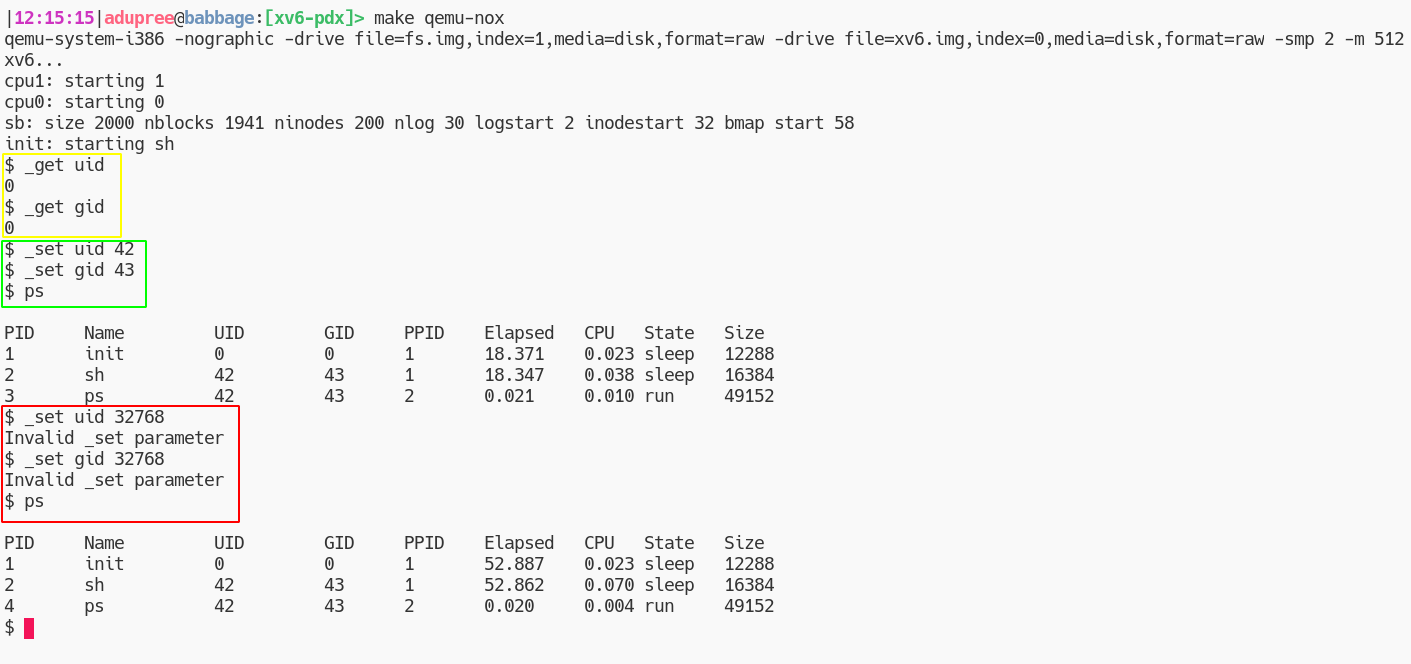
\includegraphics[width=1\linewidth]{built-in-cmds.png}
	\caption[img]{Compilation and boot with CS333\_PROJECT set to 0.}
	\label{fig:P1compileP0-1}
  \end{figure}

  The first set of commands, highlighted in the \textcolor{Yellow}{\textbf{Yellow}} box, 
  demonstrates that assertion \emph{(1)} is true. The call to \code{\_get uid} 
  and \code{\_get gid} both display \code{0} to the console because the \code{sh} process inherits from the
  \code{init} process, whose UID/GID is \code{0}. \\
  \indent Assertions \emph{(2)} and \emph{(3)} are demonstrated true in the second set of commands,
  highlighted in the \textcolor{Green}{\textbf{Green}} box. First, we set the UID/GID for 
  the \code{sh} process to 42 and 43 respectively. Then we execute the \code{ps} user program
  which will inherit the new UID/GID values from the parent \code{sh} process and then display
  the UID/GID for all system processes. \\
  \indent Finally, the commands in the \textcolor{Red}{\textbf{Red}} box demonstrate that the
  fourth assertion is also true. Attempting to set the UID or GID to 32768 results in an error
  message. Furthermore, the subsequent call to \code{ps} shows that the UID/GID of the \code{sh}
  process was not changed after the failure. 

  \noindent\textbf{Test Case:} \emph{Running the `testuidgid' test suite}
  
  \noindent\textbf{Assertions:}
  \begin{enumerate}[]
  \item Correctly set / get UID, GID, and retrieve PPID
  \item PPID for processes with no parents is properly handled
  \item Correctly handle attempting to set UID/GID to invalid values
  \item Child processes correctly inherit UID/GID values
  \end{enumerate}  
  
  \noindent\textbf{Status:} \textcolor{ForestGreen}{\textbf{PASS}}
  
  \begin{figure}[h!]
	\centering
	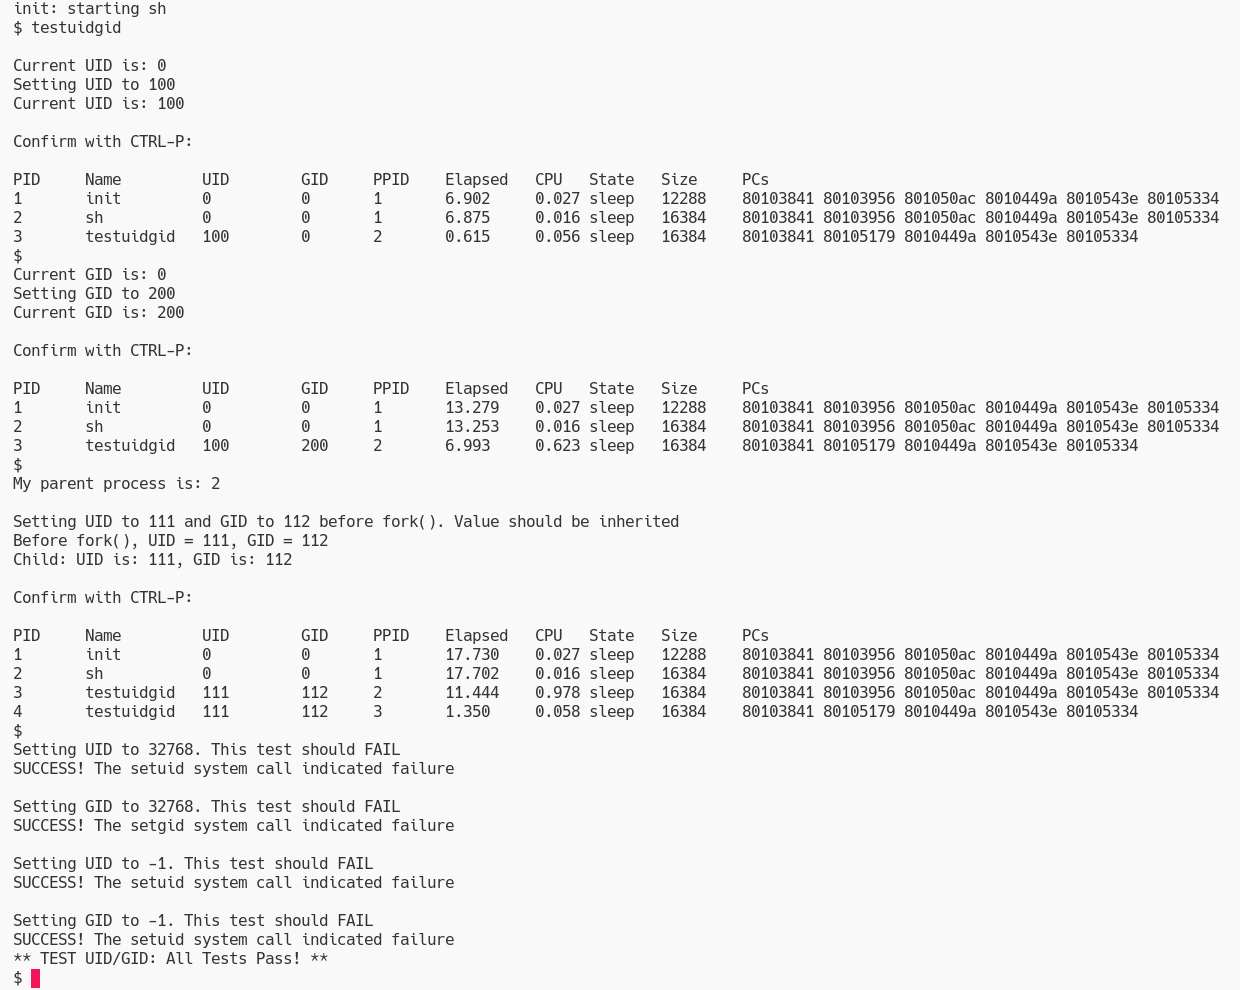
\includegraphics[width=1\linewidth]{testuidgid.png}
	\caption[img]{Compilation and boot with CS333\_PROJECT set to 0.}
	\label{fig:P1compileP0-1}
  \end{figure}

  This tests executes the provided \code{testuidgid.c} file, which was modified slightly 
  to accompany more tests. The \code{testuidgid} test suite, executes a series of tests to demonstrate that the
  UID, GID, and PPID functionality is correct. First, we set the UID of the current process
  to \code{100} and use the \code{CTRL-P} interrupt to verify the results. We then do the same
  manner of test for the GID. 

  Next we set the UID/GID to 111 and 112 respectively and fork the
  process to see if the values are correctly inherited. With \code{CTRL-P} we can see that the
  child process does indeed inherit the parents UID and GID. Furthermore, the child's PPID is 
  \code{3} which is the correct parent process ID. It's also important to note that the 
  PPID for the \code{init} process is the same as it's PID, this is becasue the \code{init}
  process does not have a parent process.

  Lastly, we attempt to set the the UID/GID to values just outside the valid boundary of 
  $0 \leq x \leq 32767$. Beacuse each attempt to set the identifier to an invalid value 
  returned failure, these tests pass. 

  \section*{Time program}
  This section presents all tests related to the \code{time} user program.
  Test cases follow closely those outlined in the rubric. \hfill \break
  
  \noindent\textbf{Test Case:} \emph{Calling time with no arguments and an invalid argument}
  
  \noindent\textbf{Assertions:}
  \begin{enumerate}[]
  \item Displays the time it execute (null) or invalid argument. 
  \item Time does not crash the kernel
  \end{enumerate}  
  
  \noindent\textbf{Status:} \textcolor{ForestGreen}{\textbf{PASS}}
  
  \begin{figure}[h!]
	\centering
	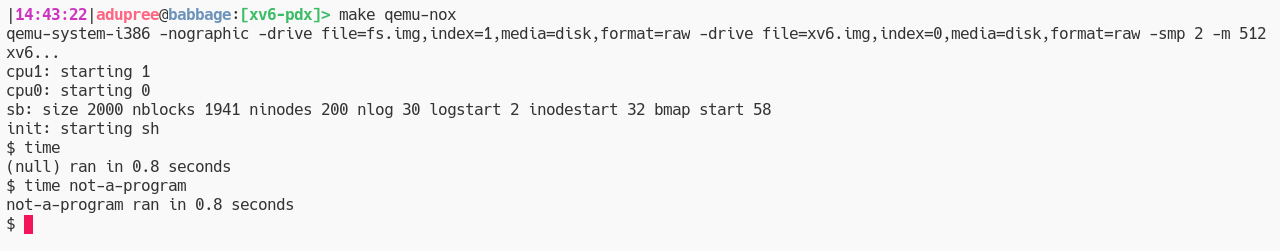
\includegraphics[width=1\linewidth]{time1.png}
	\caption[img]{Running \code{time} with no arguments and an invalid argument}
	\label{fig:P1compileP0-1}
  \end{figure}

  First, we run \code{time} with no arguments and the output matches the output provided
  in the project description. Next, when we run \code{time} with an invalid argument, the
  program displays the argument and the subsequent time. Note that both invocations resulted
  in the same time result of 0.8 seconds. This indicates that in both cases the program 
  underwent the same control flow, where the \code{exec} system call failed, and the child 
  process exited almost immediately.

  \pagebreak

  \noindent\textbf{Test Case:} \emph{Calling time with a valid command and subsequent argmuments}
  
  \noindent\textbf{Assertions:}
  \begin{enumerate}[]
  \item Time correctly executes the valid command
  \item Time correctly passes the arguments to the forked process
  \end{enumerate}  
  
  \noindent\textbf{Status:} \textcolor{ForestGreen}{\textbf{PASS}}
  
  \begin{figure}[h!]
	\centering
	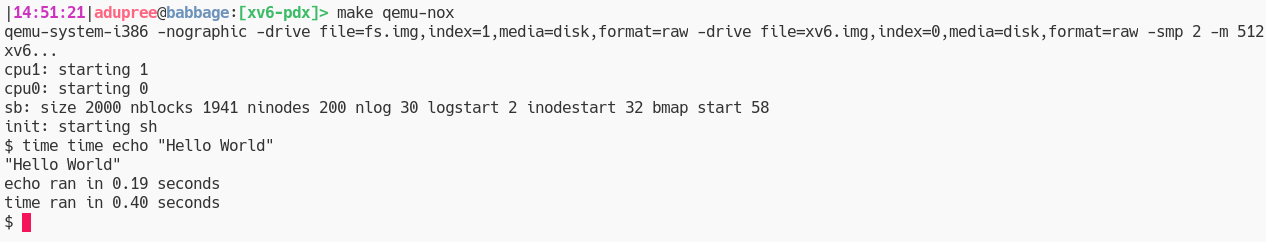
\includegraphics[width=1\linewidth]{time2.png}
	\caption[img]{Calling time with multiple commands and arguments}
	\label{fig:P1compileP0-1}
  \end{figure}

  The command \code{time time echo "Hello World"} shows that both our assertions are true. 
  First, \code{time} is executed with the arguments \code{time echo "Hello World"}. The 
  initial \code{time} process forks itself and executes the next command, \code{time}, 
  with the arguments \code{echo "Hello World"}. This process repeats itself one more time
  with the execution of the \code{echo} command with the arguments \code{"Hello World"}. 
  Finally, as the processes finish execution, the parent \code{time} processes print
  the elapsed time. Because the initial arguments perpuated isself through multiple layers
  and the correct commands were executed, we can be confident that our program is working 
  as expected.\\

  \noindent\textbf{Test Case:} \emph{Calling the time command with a long running process}

  \noindent\textbf{Assertions:}
  \begin{enumerate}[]
  \item The calculated time is accurate
  \end{enumerate}  
  
  \noindent\textbf{Status:} \textcolor{ForestGreen}{\textbf{PASS}}
  
  \begin{figure}[h!]
	\centering
	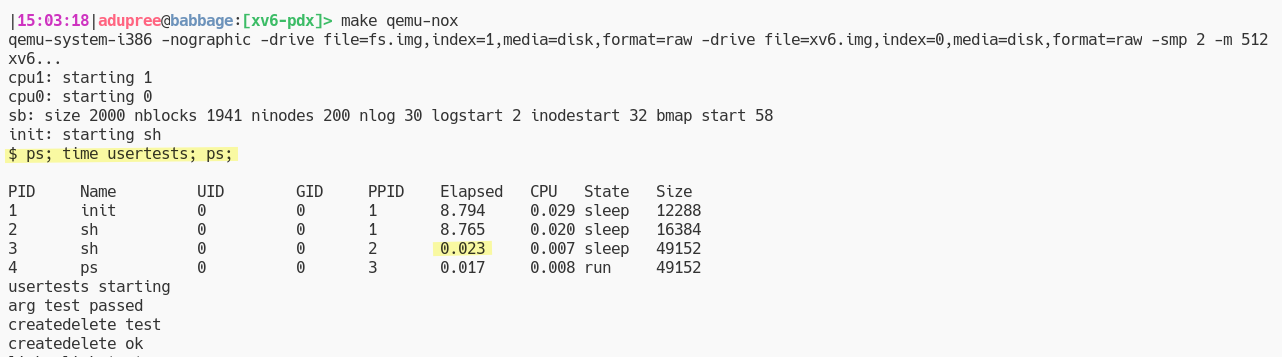
\includegraphics[width=1\linewidth]{time-invocation.png}
	\caption[img]{Invoking ps and time usertests}
	\label{fig:P1compileP0-1}
  \end{figure}

  \begin{figure}[h!]
	\centering
	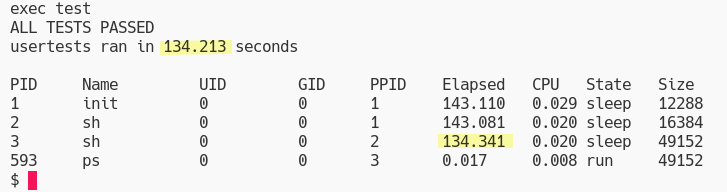
\includegraphics[width=1\linewidth]{time-result.png}
	\caption[img]{time usertests result and subsequent ps call}
	\label{fig:P1compileP0-1}
  \end{figure}

  \pagebreak

  To establish that the \code{time} command is accurate, we bound the command between
  two \code{ps} commands. As we can see the time result is nearly identical to the 
  elapsed time of the \code{sh} process that was forked to execute the command sequence.
  This strongly indicates that the calculated time is indeed accurate. It is important to note 
  that I opted to use \code{ps} over \code{date} (which was suggested in the rubric) to bound
  the command because \code{date} does not read form the \code{ticks} global variable instead 
  but instead reads time from the cmos, wich QEMU emulates. Because of this, when running the command 
  \code{date; time usertests; date;} there is a 4-5 second discrepency. As such, I wanted
  to present a test that had less ambiguity and decided to bound the command with \code{ps}. 

  \pagebreak

  \section*{Composite Test}
  The following test case executes the provided \code{p2-test} program. 
  The \code{p2-test} program is a test suite that executes a variety of project 2 related
  tests. Namely, it will test for UID/GID set, get, and inheritence. It will test the 
  \code{getprocs()} system call with an invalid array size, and with the MAX parameter
  set to 1, 16, 64, and 72 with 64 active processes running. Lastly, it will test the
  calculated CPU time for processes and the \code{time} user program. \hfill \break
  
  \noindent\textbf{Test Case:} \emph{Running the \code{p2-test} suite}
  
  \noindent\textbf{Assertions:}
  \begin{enumerate}[]
  \item Composite test runs to completion with no errors
  \end{enumerate}  
  
  \noindent\textbf{Status:} \textcolor{ForestGreen}{\textbf{PASS}}
  
  \begin{figure}[h!]
	\centering
	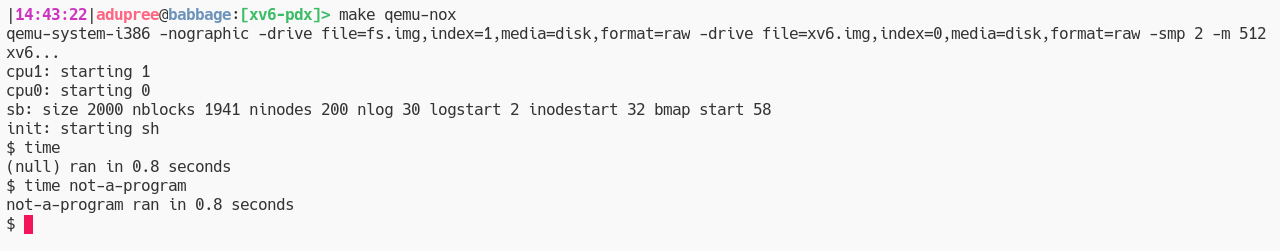
\includegraphics[width=1\linewidth]{time1.png}
	\caption[img]{Running \code{time} with no arguments and an invalid argument}
	\label{fig:P1compileP0-1}
  \end{figure}

\ifdefined \LF
} % large print end
\fi

\end{document}